%
% NOTE: This question is meant to take up one full page
%	and includes all necessary spacing.
%


Assuming the turtle is facing East, write the Python code to draw the following picture given the proper depth as input:
    \begin{itemize}
            \item depth = 0
           \\No output 
            \item depth = 1\\
            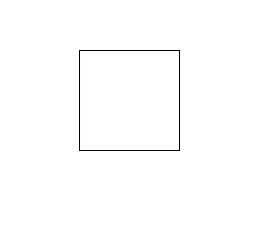
\includegraphics[scale=0.4]{other/1.png}
            \item depth = 2 \\
            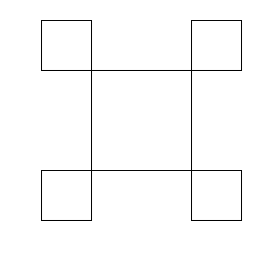
\includegraphics[scale=0.4]{other/2.png}
            \item depth = 3\\
            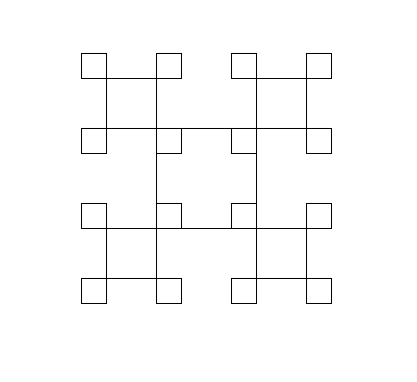
\includegraphics[scale=0.4]{other/3.png}
        \end{itemize}
    \begin{answer}

\vspace{-28pt}

    \begin{lstlisting}
       def drawSqaures( length, depth ):
           if depth <= 0:
               return
           count = 4
           while count > 0:
               turtle.forward( length )
               turtle.left( 90 )
               drawSqaures( length/2, depth-1 )
               turtle.right( 180 )
               count -= 1
        
        NOTE: Solution starts from top-left corner of the main box.
      \end{lstlisting}
     \end{answer}